% !TEX root = ../Survey.tex
We first describe general \routing schemes and two models for labeling schemes of \routing called \textit{designer port  model} and 
\textit{fixed port model}.
In Section~\ref{routing:literature} we  provide a literature review.
In Section~\ref{sec:ThorupZwick} we describe in detail the current best upper bound for routing in the designer port model due to \citeN{Thorup01}. We provide a corrected proof for this result.
In Section~\ref{sec:ThorupZwickFixedPort}  we  present a proof omitted in \citeN{Thorup01}, that shows an efficient construction of a \routing scheme for the \emph{fixed port} model.

\subsection{Introduction to routing schemes}\label{section:routing-intro}
Labeling schemes are one of many methods to maintain a \routing scheme.
A \routing scheme is a mechanism that can deliver packets of information between any two nodes in the network.
Typically, such mechanism consist of 
\begin{inparaenum} [\itshape I. \upshape)]
	\item~a \routing  function \item~the format of the address; \item~a  local labeling of the nodes; \item a message  header format, and \item~local information  to perform the computation of the \routing function \end{inparaenum}  \cite{Fraigniaud01}.
	
\routing labeling schemes produce \emph{direct}  \routing schemes, which means that the message header is fixed  once by the source host, and cannot be modified by intermediate nodes on its route to the destination.
Rather than supplying the entire path,  a node  provides only the next node to visit in order for the packet to arrive at its destination.  The local labelings of  edges from every node are identified by so called \emph{port-numbers}.
	\begin{definition}\label{dfn:port}
		Let $T=(V,E)$ be a tree with $n$ nodes, and let $u \in V$ be a node with degree $\Delta$.
		A \emph{port numbering} is an injective  function that assigns integers to the edges incident to $v$.
	\end{definition}
	
Note that a port assignment is performed  locally, and an edge can receive two different port numbers from each of its nodes.
The two main variants  considered in the literature are the  \emph{designer port} model and \emph{fixed port} model.
The former allows the encoder  to freely enumerate the  incident ports to all nodes, while the latter assumes that the port numbers are fixed by an adversary. 

\routing labeling schemes are related to two functions previously discussed in the survey, namely \ancestry and \NCA.
Unlike \ancestry, a \routing query is meaningful even for unrooted trees.
In the literature surveyed, the tree is assumed to be rooted, and for the designer port model the port number of the parent is $0$ and the port number of the heavy\footnote{A child with maximal number of  decedents.} child is $1$.
Under these assumptions, designer port \routing labeling schemes  produce labels that are able to determine \ancestry, since for an ancestry query $\la(u),\la(v)$ we  can run the \routing decoder and return true if its value is not $0$. 
Finally, we note that the  \NCAl labeling scheme presented in Theroem~\ref{thm:nca-short}  can answer designer port \routing queries, since  the labels can determine the first edge on the shortest path between the nodes queried.
		
\subsection{Literature review}\label{routing:literature}
Labeling schemes for  \routing were introduced by \citeN{peleg1999proximity}.
  \citeN{Fraigniaud01}  achieved a labeling scheme of size $3 \log n$ for the function.
 \citeN{Thorup01} presented, almost at the same time, an improvement of the label size to $(1+o(1))\log n$ for the designer port model.
\citeN{fraigniaud2002space} then showed a lower bound  for any fixed port labeling scheme for \routing of $\Omega(\log^2 n / \log \log n )$. In an experimental paper \citeN{krioukov2007compact} compared the performance of several labeling schemes for both models. Korman and Peleg~\shortcite{korman2006dynamic,korman2008improved}, studied the function in a  dynamic tree network settings, with permitted relabeling.

Unlike the situation in trees, there could be many paths between  two nodes in arbitrary graphs.
For this class of graphs, \routing schemes attempt to route the  package along a shortest, or a close-to shortest path.
The parameter measuring the quality of the path is called \textit{stretch}\footnote{Formally the stretch of a routing scheme is the worst case ratio between the length of the path obtained by the routing scheme and the length of the shortest path between the source node and the destination node.}.
\citeN{gavoille2001space} showed a lower bound implying that achieving stretch $3$ or less requires $\Omega(n)$ bits. \citeN{abraham2004compact} showed a stretch $3$  \routing scheme  with a $O(\sqrt n )$  local information stored in each node.
For surveys on \routing schemes see~\cite{gavoille2001routing}, and~\cite{Dom07}.

\subsection{Designer port model}\label{sec:ThorupZwick}
We present the proof for the following theorem. 
\begin{theorem} \label{thm:routing-upper} \cite{Thorup01} 	
	There exist a designer port model \routing labeling scheme for $Trees(n)$, denoted  \tuple{e,d}, with labels of size at most $(1+o(1)) \log n$.
\end{theorem}
We first describe the label, prove that its size is bounded, and finally describe the decoding process.

\paragraph{Label description}
Given a tree $T$, we first decompose it using the  spines decomposition defined in Section~\ref{tec:Splines}.
In this decomposition all nodes are on a  $heavy_s$ path at some stage of the decomposition.
In particular, a node $v$ of size $\size(v)$ is a member of a $heavy_s$ path at level $\LD(v)$ if $\size(v)> n/b^{\LD(v)}$.
The \emph{level} number $\LD(v)$ is in the range $\{1 \dots \log_b n\}$ and stands for  the number of iterations of the   decomposition where  $v$ is a $light_s$ node.

Similarly to the definitions   in Section~\ref{tec:heavylight}, a  node $v$ in $T$ with  $light_s$ children $v_1 \dots v_d$ has \emph{light size} $\lsize_s(v) = \sum_{i=1}^{d} size(v_i)+1$.  
We also define the \emph{light size} of a path $P = u(1) \leadsto u(k)$ as $\lsize_s(P) = \sum_{i=1}^{k} \lsize_s(u(i))$.
The collection of paths in level $i$, in decreasing order of their light size, is denoted $P^i=P^i_1 \dots P^i_l$, and the light size of $P^i$ is just the sum of their light sizes. 
The  node with the $k$'th largest light size in the path with the  $j$'th largest path size at level  $i$ is denoted $P^i_j[k]$.
See Figure~\ref{fig:routing-crazy} for a demonstration.

					\begin{figure}[!ht] 
				\centering
				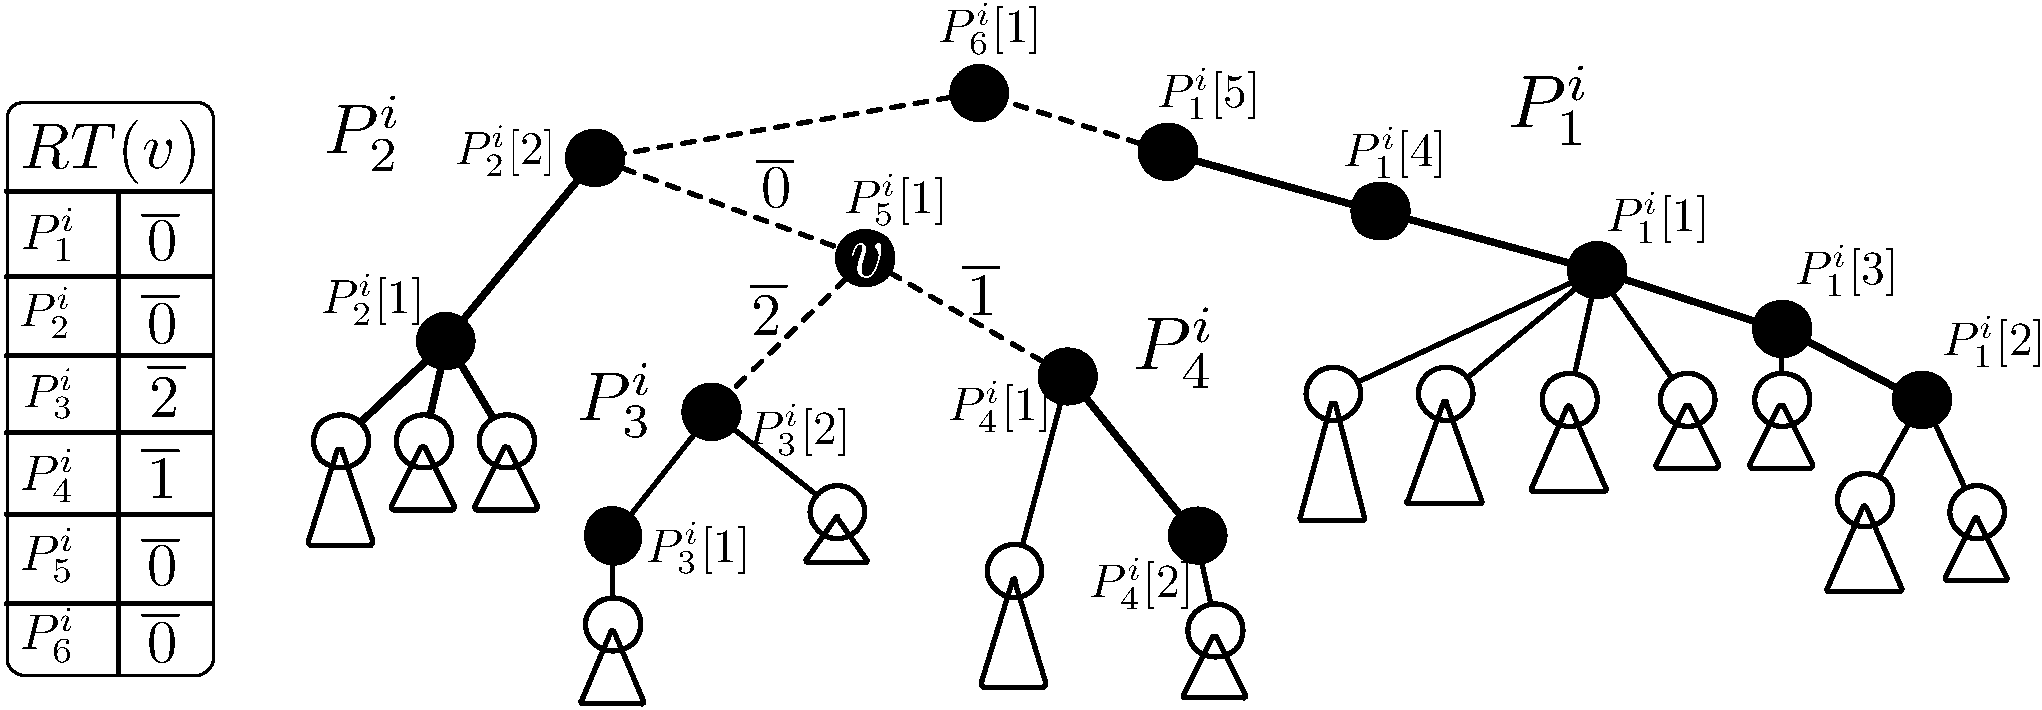
\includegraphics[width=100mm]{./Figures/Crazyrouting.pdf}
				\caption{A demonstration of naming of the  paths and $heavy_s$ nodes on level $i$ of a spines decomposition of a  subtree. 
				The thick lines are $heavy_s$ paths. The $heavy_s$ nodes are full, the $light_s$ nodes are empty, and the triangles are represent  subtrees of $light_s$ nodes.  The routing table of node $v$ to the left describes which one of the ports $\bar{0},\bar{1}$ and $\bar{2}$ it needs to traverse to arrive at nodes at other $heavy_s$ paths on level $i$. The $i$'th triplet in $\la(v)$ is $\tuple{5,1,\epsilon}$.}
				\label{fig:routing-crazy}
			\end{figure}
			

A node $v$ is assigned a two part label $\la(v)= (\Id(v),RT(v))$, described below.
The part $\Id(v)$ is, by itself, a  concatenation of triplets  of the form $\tuple{j_i,k_i,p_i}$, for $ 1 \leq i \leq  \LD(v) \leq \log_b n$, defined as follows:
 The parts $j_i$,  and $k_i$  specify $P^i_j[k]$, the $heavy_{s}$ node on level $i$ on the path  $r \leadsto v$ of maximal depth.
 We use Lemma~\ref{lemma:Gilbert} to number both $j_i$ and $k_i$.
 More specifically,  we choose  $j_i$ according to the relative contribution of  $\lsize_s(P^i_j)$ to   $\lsize_s(P^i)$, such that  $\vert j_i \vert = \log (\lsize_s(P^i)/ \lsize_s(P^i_j)) + 1$. Similarly, we choose $k_i$ according to the relative contribution of $\lsize(P^i_j[k])$ to $\lsize_s(P^i_j)$.
The part  $p_i$ is the port number used from $P^i_j[k]$ to the node $v$, which is also assigned using Lemma~\ref{lemma:Gilbert} with $\size(p_i)$ and $\lsize(P^i_j[k])$.
Note that  for the last triplet in $\Id(v)$ we use the empty string for  $p_{\LD(v)}$. 
As in Section~\ref{section:routing-intro}, the ports to  the root and the $heavy_s$ child are marked $0$ and $1$, respectively.
 Each label contains up to $\log_b n $ triplets of  three parts, where each part may be of different length.
In order to distinguish between the parts of each triplet, we store each part in $\Id(v)$ using  the suffix  code $code_1$ (see Section~\ref{sec:efficient-encoding}).
In this way a part of $m$ bits requires $m + O(\log m )$ bits, and the different parts may be concatenated.

The second part of $\la(v)$, is the level \routing table $RT(v)$ of $v$ that  contains the  ports  $v$ must use  to arrive at each of the  $heavy_{s}$ paths $P^{\LD(v)}_1 \dots P^{\LD(v)}_l$ in $v$'s level $\LD(v)$.
If $v$ is not the last node on its heavy path, then each  description concludes in traversing the path in some direction, i.e., up or down.
If $v$ is the last node, we assign the associated ports with the numbers of the ports leading to the roots of other paths in level $\LD(v)$.
This concludes the description of the label.

To compute the size of this labeling scheme we first prove the following Lemma.
\begin{lemma}\label{lemma:tikun}
$\sum_{i=1}^{\log_b n} \vert j_i \vert + \vert k_i \vert + \vert p_i \vert = \log n + O(\log_b n).$
 \end{lemma}
 
 \begin{proof}
 Let  $\tuple{j_1,k_1,p_1}$ be the first triplet in $Id(v)$ for a node $v$, and let $u$ be the light   child of  $P^1_j[k]$ to which port $p_1$ is addressed to.
  We first prove that $$\vert j_1 \vert + \vert k_1 \vert + \vert p_1 \vert \leq  \log n - \log (\size(u))+ O(1).$$
  By definition: 
  $$\vert j_1 \vert  \leq \log (n/\lsize_s(P^1_j)) +O(1) = \log n - \log (\lsize_s(P^1_j))+O(1),$$ and also 
    $$\vert k_1 \vert  \leq \log (\lsize_s(P^1_j) /\lsize_s(P^1_j[k]))+O(1) = \log (\lsize_s(P^1_j)) - \log(\lsize_s(P^1_j[k]))+O(1). $$
    Similarly, 
    $$ \vert p_1 \vert \leq \log( \lsize_s(P^1_j[k]) / \size(u) ) +O(1) =  \log( \lsize_s(P^1_j[k])) - \log (\size(u)) +O(1).$$
    Summing those inequalities we get:
    $$\vert j_1 \vert + \vert k_1 \vert + \vert p_1 \vert \leq  \log n - \log (\size(u))+ O(1),$$ as requested.
    
    Since $\lsize_s(P^2) \leq \size(u)$, we can repeat the argument so that for $w$, the light child of $P^2_j[k]$ addressed  by port $p_2$ we have:
     $$\vert j_2 \vert + \vert k_2 \vert + \vert p_2 \vert \leq  \log (\size(u)) - \log (\size(w))+ O(1).$$
     
     Summing over all the triplets, it follows that:
     $$\sum_{i=1}^{\LD(v)} \vert j_i \vert + \vert k_i \vert + \vert p_i \vert  \leq \log n +O(1) \cdot \LD(v) \leq \log n + O(\log_b n).$$
 \end{proof}

\begin{lemma} \label{lemma:routingsize}
The encoder described above produces labels of size at most $\log n + O(\log n  / \log \log n \cdot \log \log \log n)$.
\end{lemma}
\begin{proof}
 Choosing $b = \ceil{ \sqrt{\log n } }$ we can bound  the number of the  triplets  in $\Id(v)$ by  $\log_b{n} =  \frac{\log \log n}{2}$.
 The number of bits required to represent them is:
 $$\sum_{i=1}^{\log_b n} \vert j_i \vert + \vert k_i \vert + \vert p_i \vert  +O ( \sum_{i=1}^{\log_b n} \log (\vert j_i \vert)  + \log (\vert k_i \vert)  +  \log( \vert p_i \vert ) +3  ) .$$
The first sum corresponds to  the number of bits required to store the information, and the second sum is the additive number of bits required to encode each part in $code_1$. By Lemma~\ref{lemma:tikun} the first sum is bounded by  $\log n + O(\log_b n)$ bits. 
 
For brevity, we denote the number of parts by  $k= 3 \log_b n$ and the size of the $k$ parts in $\Id(v)$  by $c_1 \dots c_{3{k}}$
 Next we   bound $\sum_{i=1}^{k} \log c_i$, where $\sum_{i=1}^{k}c_i \leq  \log n + O(k)$ by Lemma~\ref{lemma:tikun}.
Since $\log$ is a concave function, we have:
$$\sum_{i=1}^{k} \log c_i \leq  k \log (\frac{\sum_{i=1}^{k} c_i}{k}) = k \log (\frac{ \log n + O(k)}{k}) \leq k \log (\frac{ \log n}{k}) +O(1)k .$$
Since $\frac{\log n}{3 \log_b n}  = \frac{\log_2 b}{3}$ the expression  can be bounded by  $O( k \log \log b+ 3 \log_b n)$, which is bounded by $O(\frac{\log n}{\log \log n}\log \log \log n).$
 

%We now prove that the $\vert RT(v) \vert $ is also $O(\log n  / \log \log n \cdot \log \log \log n)$.
To account for the size of $RT(v)$, recall that at every level of the spines decomposition there can be at most $2b-1$ paths.
Furthermore, since the ports stored lead to subtrees with at least $n/b$ nodes, it is guaranteed that each  port will be assigned an identifier with $O(\log b)$ bits. Thus, storing $RT(v)$ requires  $O( b \log b)$ bits, and  for $b = \ceil{\sqrt {\log n}}$, this can also be bounded by   $O(\frac{\log n \cdot \log \log \log n }{ \log \log n})$.
\end{proof}	 		


\paragraph{Decoding} We confirm that the information stored in the label is sufficient to determine the function \routing.
 A key observation is that while  it is not possible to  determine the rank of the a node  in its $heavy_s$ path,
 the order between two nodes on the same $heavy_s$  path can be determined.
 
Let $v$,$u$ be two nodes in $T$ with labels $\la(v) = (\Id(v),RT(v))$, $\la(u)= (\Id(u),RT(u))$ with depth  $\LD(v)$, $\LD(u)$, respectively in the recursive decomposition of $T$.
 
 If $\vert \Id(v) \vert  < \vert \Id(u) \vert $ then the decoder returns $0$, since that implies that $u$ is not an ancestor of $v$ and the path $u \leadsto v$ must begin with the edge traversing upwards from $u$.
Using the same argument,  we  return $0$ if the first $\LD(u)-1$ triplets of both $\Id(v)$ and $\Id(u)$ are not equal.
 
 Let $(path_v,node_v,edge_v)$ and $(path_u,node_u,\emptystring)$ be   triplets number $\LD(u)$ in $\Id(v)$ and $\Id(u)$, respectively.
There are three possible scenarios:
\begin{itemize}
	\item If $path_v = path_u$ and $node_v = node_u$ return $edge_v$.
	\item If $path_v = path_u$ and $node_v \neq node_u$, then determine which of $node_v$ and $node_u$ are first on the heavy path and return $0$ if the former and $1$ if the latter.
	\item If $path_v \neq path_u$ then return the edge corresponding to the traversal from $path_u$ to $path_v$ in  $RT(u)$.
\end{itemize}

		
Lemma~\ref{lemma:tikun} is a  correction to Lemma 2.4 in the  original proof in~\cite{Thorup01}.
Using similar definitions, the Lemma argues that every triplet requires at most $\log b +2$ bits. 
The term $\lsize_s(\overline{\overline{v}})$ represents the size of the subtree rooted in a  $light_s$ node at any level including the first, and  therefore  $1\leq \size(\overline{\overline{v}}) \leq n/b$. From that we get that $\log_2 \frac{n}{\lsize_s(\overline{\overline{v}})}+2 > \log_2 b +2$.
In fact the claim $\log_2 \frac{n}{\lsize_s(\overline{\overline{v}})}+2 \leq \log_2 b +2$  in~\cite{Thorup01}  holds in the opposite direction. 

 
\paragraph{Implications}		
From  this upper bound  and the recent lower bound for \NCA~\cite{Green14} it follows that any labeling scheme for \NCA is of  provably larger size than the size required for \routing.
The question of whether  the best possible lower order term is  $O(\log n / \log \log n)$ or  $O(\log \log n)$ remains open. 
The current lower bound for designer port \routing in trees stands at $\log n + O (\log \log n)$. This follows from its relationship to \ancestry labeling schemes reported earlier. Clearly, it is of great interest to prove that a larger label size is needed for \routing  than needed for  \ancestry/\siblings/\connectivity labeling schemes.


\subsection{Fixed Port Model}\label{sec:ThorupZwickFixedPort}
We now consider the fixed port  model, i.e  the model where the port numbers are chosen by an adversary. 
We provide a proof of the following result of~\cite{Thorup01} that was omitted in their paper.
\begin{theorem} \label{thm:routing-upper-fixed}  	
	There exist a fixed  port model \routing labeling scheme for $Trees(n)$, denoted  $\tuple{e,d}$, with labels of size at most $O(\log^2 n / \log \log n)$.
\end{theorem}
\begin{proof}
	The encoder operates on the tree $T$  similarly to the one for the designer port problem.
		A node $v \in T$ with label $(\Id(v),RT(v))$ is transformed in the following manner:
		We store  additional  $\log n$ bits to denote the port number assigned by the adversary to the edge in each triplet in $\Id(v)$.
		Recall that the \routing table $RT(v)$ contains at most $b$ port numbers. We store the edge numbering  assigned by the adversary for each entry in the table.
		The new $\Id(v)$ requires  additional $\log n$ bits for each of the $\log_b n$ parts, and the new $RT(v)$ requires $b  \log n$ additional bits.  Setting $b= \ceil{ \sqrt{ \log n}}$ as before,  the total new label length is bounded by $O(\log^2 n / \log \log n)$, as required.	
\end{proof}

The labeling scheme in Theorem~\ref{sec:ThorupZwickFixedPort} is asymptotically optimal in light of  the lower bound in \cite{fraigniaud2002space}. An alternative proof for the existence  of such a labeling scheme is  given in~\cite{Fraigniaud01}.



%\paragraph{Upper bound}
%
%
%\paragraph{Lower bound}
%Fraigniaud and Gavoille proved that any labeling scheme supporting the function is of size $\Omega(\log^2 n / \log \log n)$.
%More specifically, they construct a family of trees and define a relaxed query for which the bound still holds.
%The authors consider a full k-ary tree, where $k= (\log \sqrt n / \log \log \sqrt n)-1$ and  every internal node has $\sqrt n$ leaves attached, where the height of the tree is  $h = \log \sqrt n / \log \log \sqrt n$. 
%The proof is inductive over a series of k-ary trees over varying $h$, and decreasing number of leaves per node.
%
%A key observation is that once the port assignment of the ports from the root is set, no two trees can have the exact same labels.

%The authors show that $\la^t$ 






	



	